\documentclass[twoside, 12pt, a4paper]{article}
%\include{IAP_References.bib}
% List Of Packages
\usepackage{geometry, graphicx, color, fancyhdr, setspace, caption, url}
\usepackage{psfrag,amsbsy,amsmath,textcomp,enumerate}
\usepackage[font=footnotesize]{caption}
\usepackage[nottoc,numbib]{tocbibind}
\usepackage[hidelinks]{hyperref}
\usepackage{multirow}
\usepackage{makecell}
\usepackage{float}
\usepackage{subfig}
\usepackage{setspace}
\usepackage{notoccite}
%\usepackage{natbib}
% Define Use Of Packages
% Geometry
\geometry{margin = 2cm}
\newenvironment{where}{\noindent{}where\begin{itemize}}{\end{itemize}}
\renewcommand{\refname}{REFERENCES}
\renewcommand{\contentsname}{TABLE OF CONTENTS}
%\renewcommand{\listfigurename}{LIST OF FIGURES}
%\renewcommand{\listtablename}{LIST OF TABLES}
% Enter Information
\newenvironment{myindentpar}[1]%
{\begin{list}{}%
		{\setlength{\leftmargin}{#1}}%
		\item[]%
	}
	{\end{list}}

% Fancyhdr
\pagestyle{fancy}
\fancyhead[R]{3806ICT   --Robotics, Agents and Reasoning, Trimester 1, 2021}
\fancyhead[L]{}
\fancyfoot[LE,RO]{\thepage}
\fancyfoot[LO]{Ryan Williamson, Connor Forbes}       % put your names here for fancy footer
\fancyfoot[RE]{Your Title}            % put title here for fancy header
\fancyfoot[C]{}
\renewcommand{\footrulewidth}{0.4pt}

%\bibliographystyle{IEEE}

% Begin The Document
\begin{document}
\begin{titlepage}
\begin{flushright}
	
\includegraphics[height=60px]{griffithlogo.png}
\end{flushright}
\begin{large}
\textbf{Griffith School of Information Technology}\\
\textbf{Griffith University}

\vspace*{8mm}

\textbf{3806ICT \, -- Robotics, Agents and Reasoning}\\
\textbf{Trimester 1, 2021}
\end{large}

\vspace*{15mm}

\begin{Huge}
\textbf{Grid World Maze Runner}
\end{Huge}

\vspace*{5mm}
\begin{large}


\vspace*{8mm}

\textbf{Ryan Williamson , s5135470}\\
\textbf{Connor Forbes , ss5068337}

\vspace*{8mm}
\begin{myindentpar}{2cm}
 We, by signing this page, declare that the work presented in this report is all work done by us, unless appropriate reference has been made to the work of others. I acknowledge that should this not be the case the report will receive zero marks and due action may be taken.
\end{myindentpar}

\vspace{20mm}
\textbf{Submitted on: \underline{\hspace{50mm}  } }\\

\textbf{Mark Received: \underline{\hspace{50mm}  }  }

\end{large}


\vfill

\end{titlepage}
%-----------------------------------------------------------------------------------------

%next four lines create blank page
%\pagebreak
%\pagestyle{empty}
%\textcolor{white}{This is a blank page}
%\pagebreak

% Contents page

\pagestyle{fancy}
\fancyfoot[C]{\thepage}
\fancyfoot[L,R]{}
\pagenumbering{roman}
\setcounter{page}{1}

\newpage

%\cleardoublepage
%\phantomsection 

% ----------------------------------------------------------------
\tableofcontents


%\listoffigures
%\listoftables

% ----------------------------------------------------------------
%Document content goes here.
\newpage
\pagenumbering{arabic}
\setcounter{page}{1}
\pagestyle{fancy}

\fancyfoot[LE,RO]{\thepage}
\fancyfoot[LO]{Ryan Williamson, Connor Forbes}                    % insert names for footer here
\fancyfoot[C]{}
\section{Abstract}

\section{Model the Grid World in PAT}  \label{CSys_AandD}

\subsection{World Representation}
Before the Grid World can be modelled with PAT each point needs to be parameterised as an integer as global constants can only represent boolean or integer values.This conversion is only required for PAT's internal computation and for readability convention will still be maintained. Each point within the grid world as been converted as per the following:
\begin{itemize}
\item  \textbf{‘O’ for open space -} Modelled as a the integer 3
\item  \textbf{‘H’ for a wall -} Modelled as the integer 2
\item \textbf{‘G’ for the goal location -} Modelled as the integer 1   
\item  \textbf{‘S’ for the starting location - }Modelled as the integer 0
\end {itemize}
An example 10x10 grid world has been generated and can be seen below along with the PAT's internal representation of the world. 
\begin{figure}[ht]%
    \centering
    \subfloat[\centering Readable Grid World Representation]{{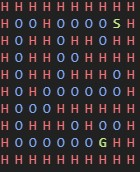
\includegraphics[width=5cm]{GridWorld10x10.jpg} }}%
    \qquad
    \subfloat[\centering Internal PAT Representation]{{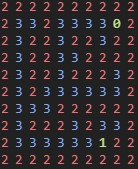
\includegraphics[width=5cm]{GridWorld10x10_PAT.jpg} }}%
    \caption{5x5 Grid World Representation}%
    \label{fig:example}%
\end{figure}
\subsection{Game Choices}
Four guarded choices are available at each game state that can be taken to move the current position around the maze, the guarded process serves to prevent any illegitimate states from being reached where the position is outside the bounds of the maze. \\
\begin{itemize}
 \item \textbf{Move Up -} Move the current location up one row
 \item \textbf{Move Down -} Move the current location down one row
 \item \textbf{Move Left -} Move the current location left one column
 \item \textbf{Move Right -} Move the current location right one column
\end{itemize}
\subsection{Assertion}
With the Game choices and actions modelled, an assertion can be made that the goal state is reachable for the current board. The goal state can be defined as \\
\begin{equation}
Goal = Board[Row][Col] == G
\end{equation}
Where Row and Col are the current position, meaning that the state has traversed through the maze from the starting point to the end location.
\subsection{Model Verification Testing}
Using PAT's inbuilt model verification tool and the Game Choice, World Representation and Assertion defined the model checker can run to determine if the current maze is indeed solvable and the resultant optimal path. The below optimal path has been given for the grid world defined within Figure 1, the time taken to calculate the path was 0.0004949s\\
\begin{center}
\begin{math}
go\_left -> go\_left -> go\_left -> go\_left -> go\_down -> go\_down -> go\_down -> go\_down -> go\_left -> go\_down -> go\_left -> go\_left -> go\_down -> go\_down -> go\_right -> go\_right -> go\_right -> go\_right -> go\_right -> go\_right
\end{math}
\end{center}

<<<<<<< HEAD
\section{Model the Grid World Maze for RL} \label{ModelRL}
Reinforcement Learning is an unsupervised learning method where some states, transistions and actions have a corrosponding rewards of actions and then given a goal will determine the method to maximise the reward. This method of unsupervised learning
=======
\section{Model the Grid World Maze for RL}
A reinforcement learning model for a Grid World Maze Runner has been developed within python, seperated into two seperate stages the 

>>>>>>> e21172f99685acd51298e01fca4036c4e66fe8ed
\section{Parameterise the Grid World}
For the maze generation, a variation of the Randomized Prim’s Algorithm was implemented to generate the maze. The algorithm works as follows:
\begin{enumerate}
\item Start with a NxN maze full of univisited points (U)
\item Pick a random cell, mark it as an open space (O) and mark the four directly adjacent (top, left, right, bottom) cells as walls (H) and add to the list of walls
\item While there are walls in the list:
\begin{enumerate}
\item Randomly pick a wall from the list and check how many adjacent cells are open spaces (O). If only one of the four surrounding cells is an open space then:
\begin{enumerate}
\item Mark the wall as an open space (O) and remove from the list of walls
\item Mark the surrounding unvisited cells (U) as walls (H) and add to the list of walls
\end{enumerate}
\item Else:
\begin{enumerate}
\item Remove the wall from the list of walls
\end{enumerate}
\end{enumerate}
\item Once iteration is complete, mark the remaining unvisited cells as walls
\item Add a starting point (S) randomly at either the top left or top right open space (O) in the maze
\item Add the goal point (G) randomly at either the bottom left or bottom right open space (O) in the maze
\end{enumerate}
The above algorithm will always result in a closed maze which contains an open path from the starting point (S) to the goal (G). Any size maze can be generated by providing the with and height as arguments when running the file from the command line (e.g. `python ./grid-world-generation.py 15 15` for a 15 by 15 maze)

\section{Translate the Grid World to a PAT Model and RL Model}
Slight modifcations are required to convert the generated maze world from the generated output to eligible PAT and RL models. Extending on the end of the maze generation program two text files are created within the Mazes subdirectory, first the PAT model is written in the following format:
\begin{itemize}
 \item Define the starting X position
 \item Define the starting Y position
 \item Define the width of the grid world
 \item Define the height of the grid world
 \item Define the generated maze as a 1D array
\end{itemize}
These items are exported to a .csp file that can be then imported to the PAT model checker for verification, these parameters must also be removed from the orginal model to prevent overwriting the variables. Following from this the RL model is then written to a .txt file, the RL model only requires the generated maze world as a one dimensional array with no other defining variables. No modification is requried as the initial model as RL was designed to read the flattened maze array from a text file.

\section{PAT vs RL for Maze Runner}
An experiment has been conducted to compare PAT model verification vs Reinforcement Learning in the domain of the maze runner. The experiment will be conducted fairly by testing the models on randomly generated mazes of varying size, starting from 5x5 up to 200x200. Identical grids will be used for comparison with the times for each model to run. The following parameters will be used for comparison:
\begin {itemize}
\item \textbf{Time Taken -} How long for the model to determine the optimal path
\item \textbf{Length of Path -} How long the optimal path is
\end {itemize}
In order to form a fair comparison the training time required for reinforcement learning will also be measured and factored in as it is a requirement prior to the model running. As reinforcement learning's performance can also be heavily modifed by the identified tuning parameters these will also remain constant throughout experimentation, the same values identified within Section\ref{ModelRL} will be used.  The experiment will be completed across seven different generated mazes, beginning with smaller mazes and then spiradically increasing to get a broad overview how each model works as the complexity significantly increases. A visualisation of the generated mazes has been attached within Appendix \ref{appendix:a}.  The table below shows the collected results from the experimentation:


\begin{table}[ht]
\begin {center}
\begin{tabular}{ | c | c | c | c | c |}

\hline
 \textbf{Maze Size} & \textbf{ Time Taken (s)} &  \textbf{Optimal Path Length} &  \textbf{Training Time (s)} \\
\hline
5x5 		& 0.0000	&6	 &0.21\\
10x10 	& 0.0010	&14	 &0.52\\
20x20 	& 0.0010	&33	 &2.19\\
40x40		& 0.0010	&76	 &8.51\\
60x60 	& 0.0190	&Did not complete	 &23.06\\
100x100	& 0.0190	&Did not complete	 &22.94\\
200x200	& 0.0230	&Did not complete	 &23.24\\
\hline
\end {tabular}
\caption{\label{tab:table-name}Reinforcement Learning Results}
\end {center}
\end{table}



\begin{table}[ht]
\begin {center}
\begin{tabular}{ | c | c | c | c | c |}

\hline
 \textbf{Maze Size} & \textbf{ Time Taken (s)} &  \textbf{Optimal Path Length}  \\
\hline
5x5 		& 0.0098863	& 6	 \\
10x10 	& 0.0007578	& 14	 \\
20x20 	& 0.0049444 & 33	 \\
40x40		& 0.0500344	& 76	 \\
60x60 	& 0.1773686	& 177	 \\
100x100	& 0.7564199	& 228	 \\
200x200	& 8.874657	& 476	 \\
\hline
\end {tabular}
\caption{\label{tab:table-name}PAT Verfication Results}
\end {center}
\end{table}
As can be seen, the PAT model verification performs significantly better in all aspects of testing. Without modfiication to the tuning parameters for larger grid sizes reinforcement learning begins to struggle immensly with exploring enough of the state space to reach the goal location and properly populate enough Q values. With the drastic increases in training time as the grid sizes increases reinforcement learning becomes extremely undesirable for model verification.
%\section {REFERENCES}

\bibliographystyle{ieeetr}
\bibliography{CSYS_References}

\newpage
\appendix
\section{Appendix: Tested Maze Visualisations} \label{appendix:a}

\begin{figure}[ht]
\begin{center}
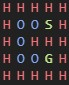
\includegraphics[width=3cm]{5x5.jpg} 
\caption{\label{tab:table-name}5x5 Maze}

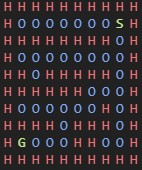
\includegraphics[width=3cm]{10x10.jpg} 
\caption{\label{tab:table-name}10x10 Maze}

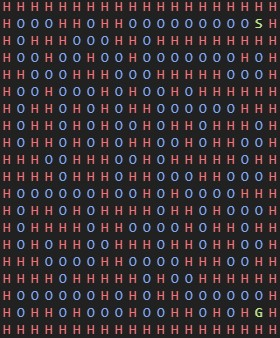
\includegraphics[width=8cm]{20x20.jpg} 
\caption{\label{tab:table-name}20x20 Maze}
\end {center}
\end{figure}

\begin{figure}[ht]
\begin{center}
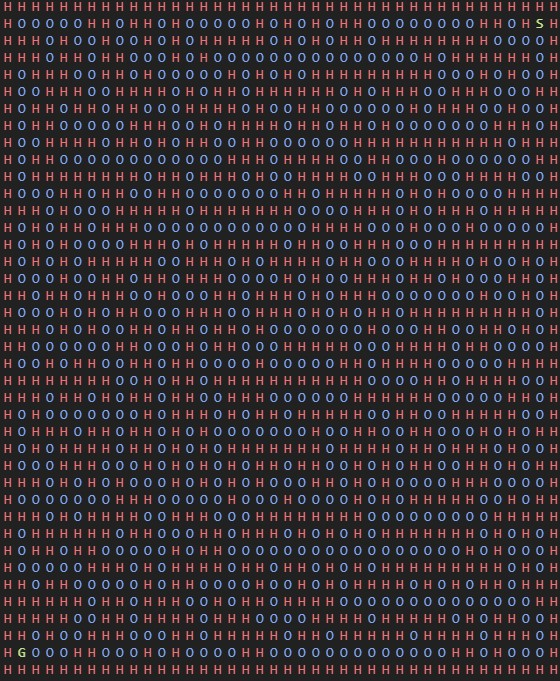
\includegraphics[width=10cm]{40x40.jpg} 
\caption{\label{tab:table-name}40x40 Maze}

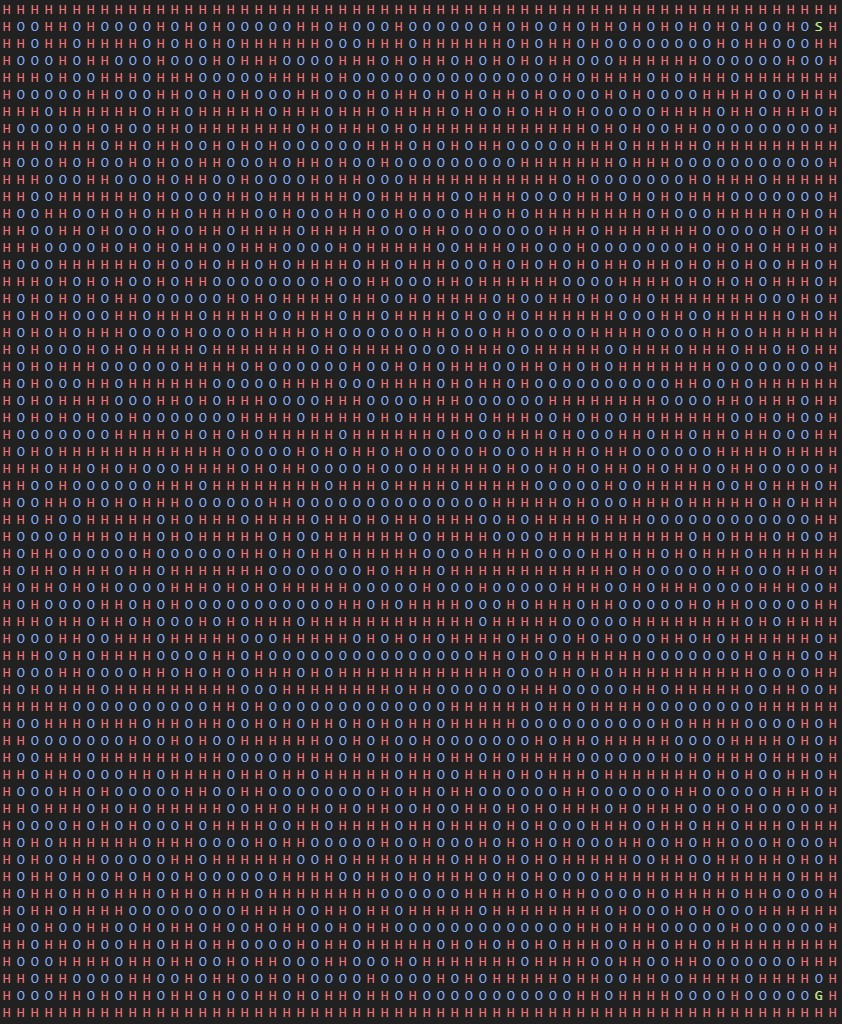
\includegraphics[width=10cm]{60x60.jpg} 
\caption{\label{tab:table-name}60x60 Maze}
\end {center}
\end{figure}

\end{document}
